
Test definition and execution is an essential but time-consuming task during system development. To speed up the process, model-based testing and other related approaches propose to select abstract test cases and to automatically concretize them, based on mapping information provided by the test engineer. This mapping may take one of the following forms \cite{Utting2007}:
\begin{inparaenum}[(i)]
\item an adapter which interprets the actions and assertions of the abstract test case and execute them on the SUT;
\item a transformation from the abstract test cases to code executable directly on the SUT; or
\item a mixture of the above two.
\end{inparaenum}
In this last case, an \gls{abstract test case} is transformed into executable code which uses an intermediate adapter (like an intermediate library for instance) to bridge the gap between the test case and the \gls{SUT}. 

In this chapter, we describe the \acrfull{AbsCon} developed by Jeremy Vanhecke \cite{Vanhecke2016} during his master thesis, we co-supervised with Dr. Gilles Perrouin and Prof. Patrick Heymans. AbsCon is defined as a QTaste \cite{qtaste} plugin, an open-source industrial data-driven test case definition and execution environment, used to perform black-box testing on various kinds of systems. QTaste abstracts the SUT's interface by using an adapter called \emph{test API}, test cases are written in Python where the operations on and the readings from the SUT's interface are encapsulated into calls to the test API dedicated to the kind of the SUT. 

For instance, to test a Web-application, QTaste encapsulates the access to the elements of the Web page in a Web test API which is responsible to perform the effective Selenium (a popular Web browser automation tool \cite{selenium}) calls. After considering different options, we chose to define AbsCon as a QTaste plugin for the following reasons:
\begin{inparaenum}[(i)]
	\item QTaste is an open source industrial tool, used to test various kinds of systems, from Web-applications to mobile applications and even cyber-physical systems \cite{Doucet2014}, thanks to its test API adaptation mechanism;
	\item plugin development is already included in QTaste and this architecture was suggested by a QTaste developer;
	\item the inital goal of AbsCon was to concretize abstract test cases selected by \gls{VIBeS} using additional mapping information. To this end, abstract test cases are defined in AbsCon using an XML file, where each test case is a sequence of actions and assertions on the SUT. But this definition is not specific to VIBeS, it also allows QTaste test engineers to define test cases in a more abstract and systematic fashion (rather than directly Python scripts), as long as they follow the same pattern (\ie sequences of assertions and actions).
\end{inparaenum}

The remainder of this chapter is as follows: Section \ref{sec:abscon:qtaste} gives a general description of the QTaste environment, Section \ref{sec:abscon:abscon} describes AbsCon's \gls{concretization} process as well as the required mapping information, Section \ref{sec:abscon:architecture} presents AbsCon's implementation, advantages and limitations are discussed in Section \ref{sec:abscon:discussion}, Section \ref{sec:abscon:relatedwork} discusses related work. Finally, Section \ref{sec:abscon:conclusion} wraps up the chapter and presents some perspectives.


%%%%%%%%%%%%%%%%%%%%%%%%%%%%%%%%%%%%%%%%%%%%%%
\section{Test automation using QTaste}
%%%%%%%%%%%%%%%%%%%%%%%%%%%%%%%%%%%%%%%%%%%%%%

\label{sec:abscon:qtaste}

The \acrfull{QTaste} \cite{qtaste} is an open source functional and non-functional black-box test environment developed in Java and Python. It has been originally developed by Qspin Experts\footnote{\url{http://www.qspin.be}} in order to automate testing process of medical cyber-physical systems developed by IBA\footnote{\url{https://iba-worldwide.com}} and used for proton therapy. 
Since its inception, QTaste has been extended to support different kinds of SUTs, like Web-applications, mobile applications, or more classical desktop applications \cite{Doucet2014}. It is released as an open source project on GitHub under GNU GPL 3.0 license \cite{qtaste}. 

%------------------------------------------------
\subsection{Overview of the QTaste environment}
%------------------------------------------------

QTaste follows the data-driven testing philosophy \cite{Williams2007}: data used by the tests are externalized in order to allow test cases parametrization. Each test case is written in Python and describes a sequence of steps, \ie \emph{operations} executed by the SUT or \emph{verifications} of the outputs produced by this SUT, using the given data as input. For instance, when testing a form which values are recorded in a database, one test case fills the form with the given data and check that the values are effectively recorded in the database. This test case is repeated with different values (\eg positive, null, and negative values for numeric fields) specified in a separate CSV file and automatically executed by QTaste on the SUT. 


\paragraph{QTaste adapter mechanism:}
%------------------------------------

QTaste provides \textit{test APIs} which communicate with the \gls{SUT} and manage the  operations executions and/or SUT's outputs reading. Each test API consists in a Java interface, defining the operations and information accessible by the test cases, and a Java implementation of this interface which manages communication with the SUT. 
This mechanism allows QTaste to test a large variety of systems: Web-applications using a Selenium-based test API, hardware components with dedicated API, or any other kind of system for which a test API may be developed. The test API, together with the configuration of the SUT instance is called a \emph{Testbed}: this mechanism allows to write test cases independently from the execution environment, using only test (and standard Python) API(s). 
Once all the test cases have been executed, QTaste generates a summary report, with the number of success and fails, the Testbed used, for each test case, the CSV lines used, \etc


\paragraph{Example:}
%------------------------------------

\begin{lstlisting}[language=Python,
float,
label=lst:abscon:testcase,
caption={Google search test case}]
from qtaste import *

api = testAPI.getSelenium(INSTANCE_ID='Google')(*@\label{lst:abscon:testcase:selenium}@*)

def init():(*@\label{lst:abscon:testcase:init}@*)
	api.openBrowser(testData.getValue("BROWSER"))(*@\label{lst:abscon:testcase:openbrowser}@*)
	api.windowMaximize()
	api.open("https://www.google.be/") (*@\label{lst:abscon:testcase:openurl}@*)
	api.waitForPageToLoad("15000") 
	if api.getTitle() != "Google": (*@\label{lst:abscon:testcase:checktitle}\label{lst:abscon:testcase:gettitle}@*)
		testAPI.stopTest(Status.FAIL)
    
def searchAndClick():(*@\label{lst:abscon:testcase:searchandclick}@*)
	api.type("id=lst-ib", testData.getValue("SEARCHVALUE"))(*@\label{lst:abscon:testcase:type}@*)  
	api.clickAt("name=btnK", "0.0" )(*@\label{lst:abscon:testcase:click1}@*)
	api.waitForPageToLoad("15000")
	api.click("link=" + testData.getValue("LINKTOCLICK"))(*@\label{lst:abscon:testcase:click2}@*)
	if api.getTitle() != testData.getValue("LINKTITLE"): (*@\label{lst:abscon:testcase:checklinktitle}@*)
		testAPI.stopTest(Status.FAIL)
		
def exit():(*@\label{lst:abscon:testcase:exit}@*)
	api.stop()(*@\label{lst:abscon:testcase:stopbrowser}@*)

doStep(init)(*@\label{lst:abscon:testcase:dostep1}@*)
doStep(searchAndClick)(*@\label{lst:abscon:testcase:dostep2}@*)
doStep(exit)(*@\label{lst:abscon:testcase:dostep3}@*)
\end{lstlisting}

Listing \ref{lst:abscon:testcase} presents a (simplified) test case for the Google search engine that is executed for each line of the external CSV file. It launches a Web browser and connects to the Google search website, fills the search field with a string, and click on a specified link. 
Line \ref{lst:abscon:testcase:selenium} creates a Selenium instance test API, which manages the connection to the browser; 
lines \ref{lst:abscon:testcase:init}, \ref{lst:abscon:testcase:searchandclick} and \ref{lst:abscon:testcase:exit} declare the steps of this test case, called at lines \ref{lst:abscon:testcase:dostep1}, \ref{lst:abscon:testcase:dostep2}, and \ref{lst:abscon:testcase:dostep3}; 
explanations about each step is given as a comment in Python format (not shown here) and is used during the generation of the test reports.
At each step, the test API instance is used to manipulate the browser user interface (lines \ref{lst:abscon:testcase:openbrowser} to \ref{lst:abscon:testcase:gettitle}, \ref{lst:abscon:testcase:type} to \ref{lst:abscon:testcase:checklinktitle}, and \ref{lst:abscon:testcase:stopbrowser}) according to the data provided in the external CSV file (identified by column names at lines \ref{lst:abscon:testcase:openbrowser}, \ref{lst:abscon:testcase:type}, \ref{lst:abscon:testcase:click2}, and \ref{lst:abscon:testcase:checklinktitle}). 
Finally, each step may check assertions on the outputs of the browser to validate the execution (lines \ref{lst:abscon:testcase:checktitle} and \ref{lst:abscon:testcase:checklinktitle}).


%---------------------------------------
\subsection{Advantages and limitations}
%---------------------------------------

The main advantage of QTaste is the test API mechanism, allowing test cases to manipulate a large variety of SUTs using a general purpose programming language: Python. Expressing test cases using a general purpose and popular programming language like Python benefits from the large number of available Python libraries. This can be very handful when writing test cases in order to perform more complex operations or access external resources. The environment provides extensibility mechanisms to the test engineers in order to write dedicated adapters between QTaste and SUTs, and describes the usage of those adapters in a test API. Coupled to the externalisation of data and SUT's configuration, it improves test cases \emph{reusability} and \emph{automation} of the test process \cite{Utting2007}. 

As it works as a black-box test environment, QTaste access the SUT through its interface, manipulated by the test cases trough the test API. This means that whenever the interface and/or the test API evolve, all the test cases using this interface and/or modified test API are impacted, increasing \emph{maintenance cost} \cite{Utting2007}. AbsCon provides an additional abstraction layer separating the different concerns thus reducing maintenance costs when combined with abstract test cases as presented in the next section.   


%%%%%%%%%%%%%%%%%%%%%%%%%%%%%%%%%%%%%%%%%%%%%%%%%%%%%%%%
\section{Test cases concretization}
%%%%%%%%%%%%%%%%%%%%%%%%%%%%%%%%%%%%%%%%%%%%%%%%%%%%%%%%

\label{sec:abscon:abscon}

\begin{figure}
	\centering
	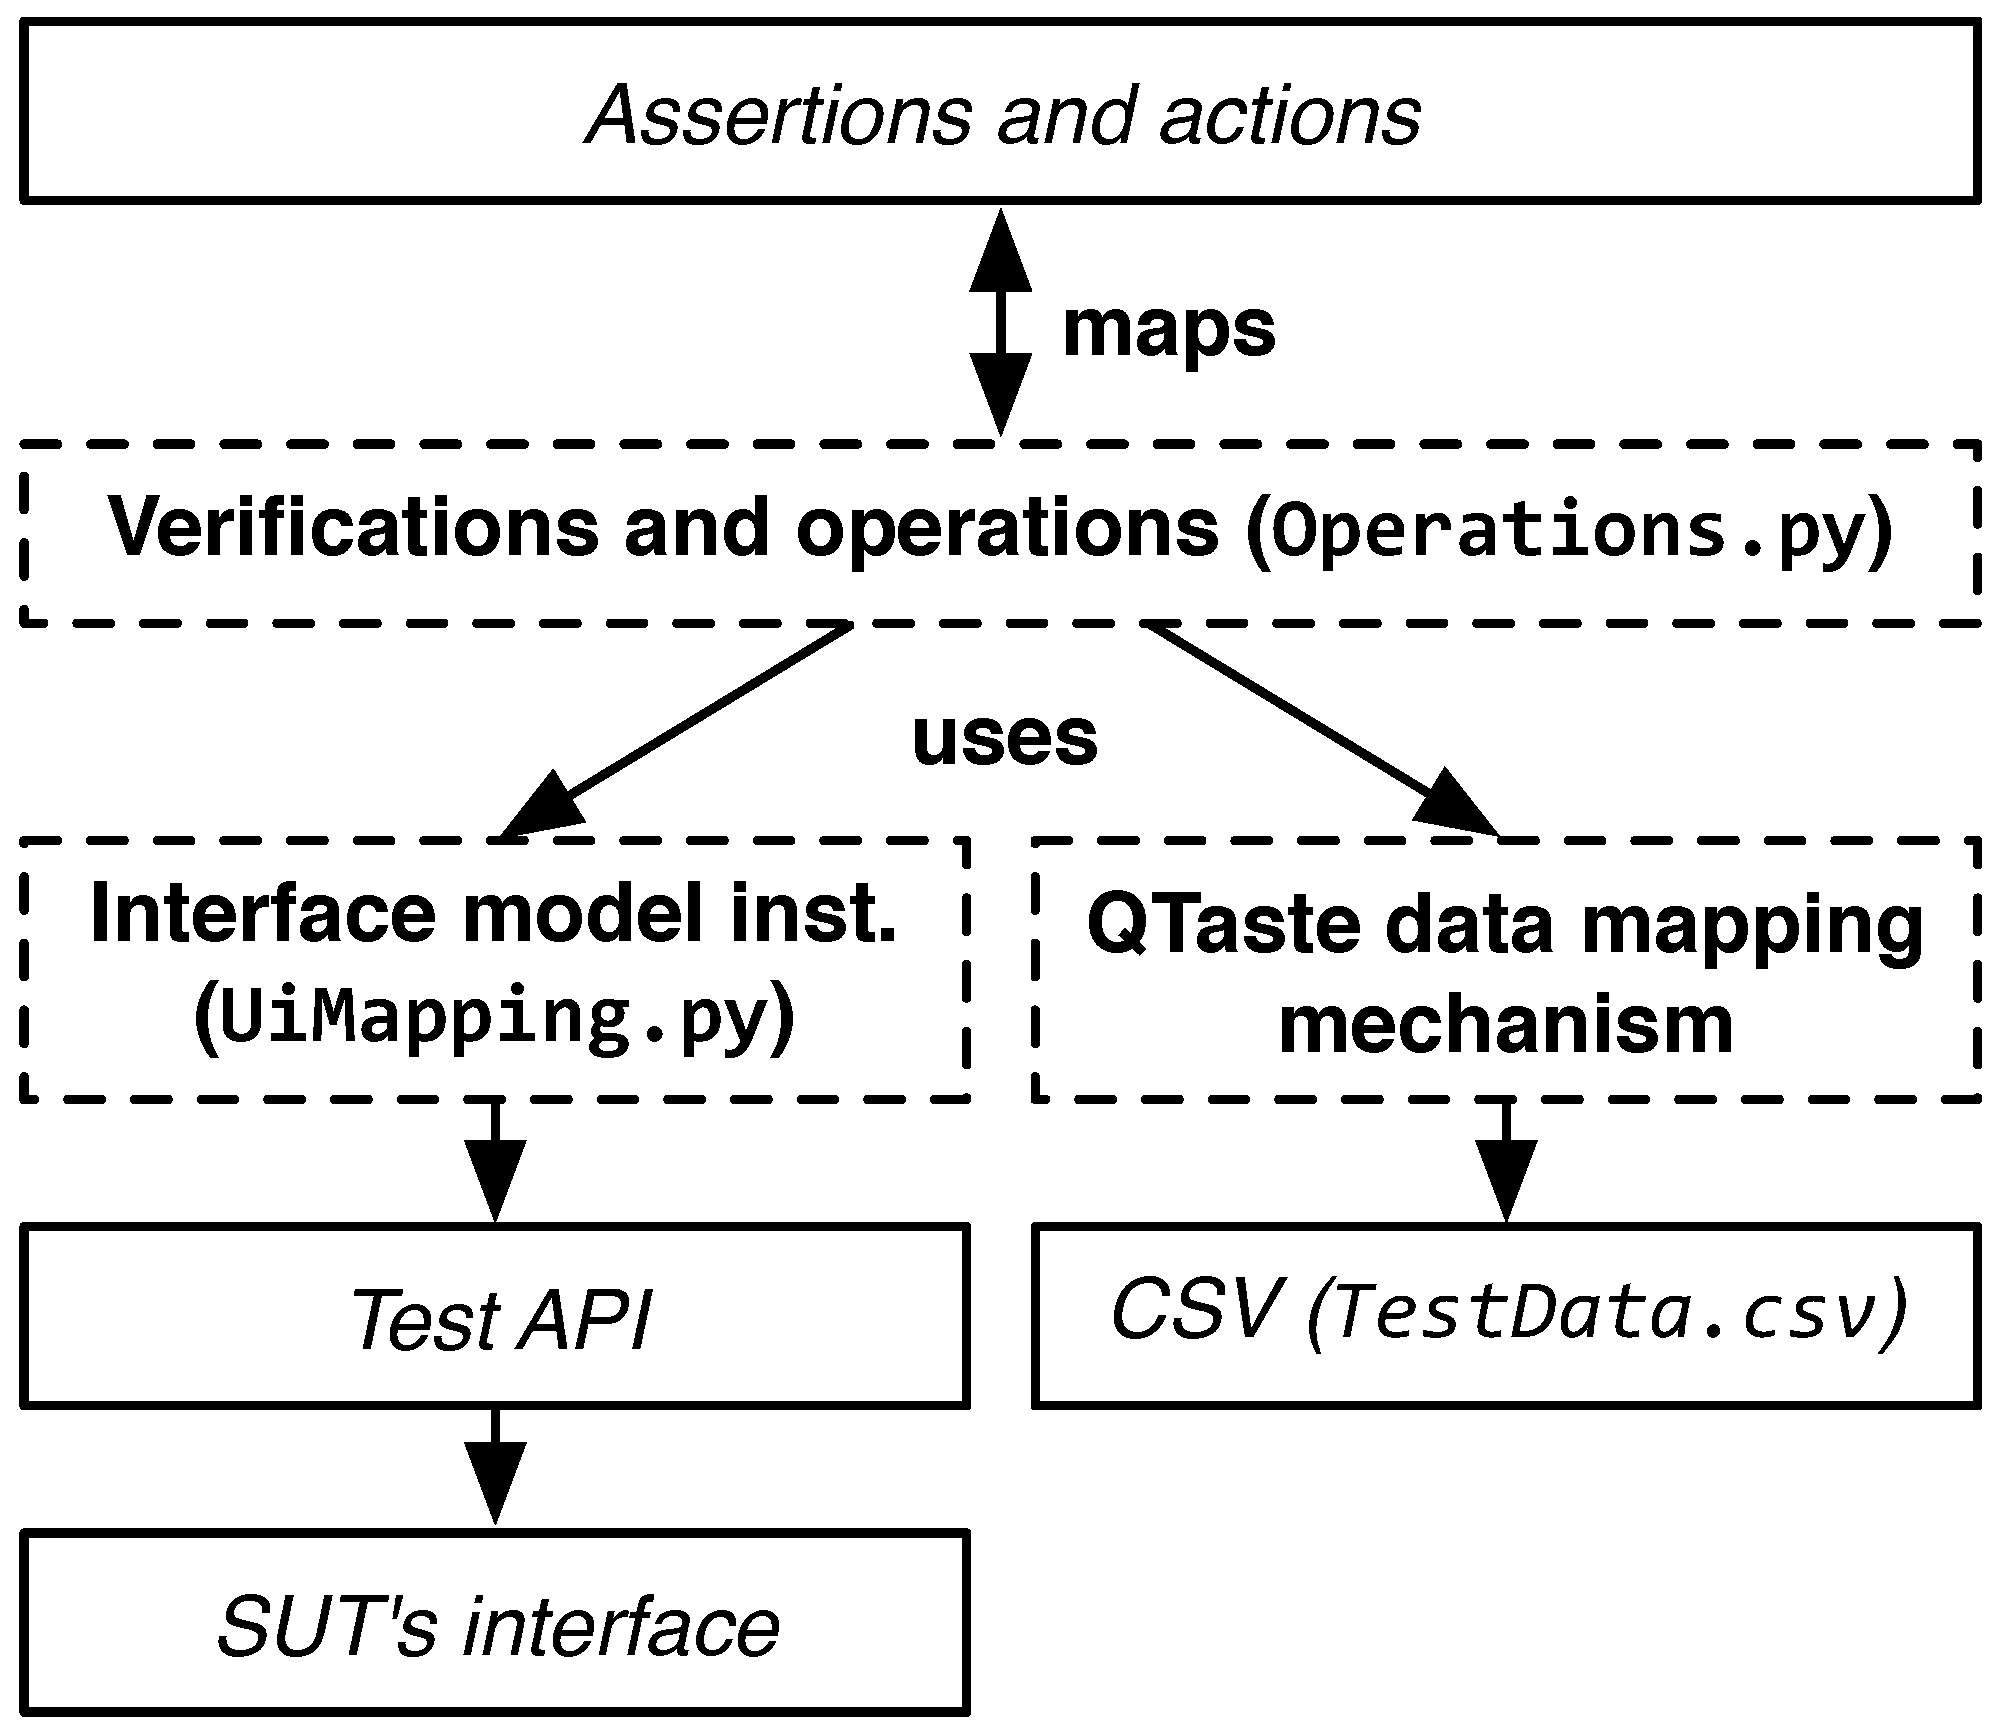
\includegraphics[width=0.33\textwidth]{abscon-mappings}
	\caption{Mappings in AbsCon}
	\label{fig:abscon:mappings}
\end{figure}

\gls{AbsCon} was originally developed to support \gls{abstract test case} \gls{concretization} \cite{Vanhecke2016}. In AbsCon, an abstract test case is a sequence of abstract \emph{assertions} and \emph{actions}, usually automatically derived by a model-based testing tool \cite{Utting2007}: VIBeS in this case \cite{vibes}. To bridge the gap between VIBeS and AbsCon, abstract test cases produced by VIBeS are enriched with the intermediate states (representing assertions on the system's state) visited when executing the abstract test case. This modification is coherent with our assumption that the behavioural model used to select  abstract test cases is deterministic.
 
The concretization process translates the abstract test case into a (concrete) test case executable by  QTaste: (resp.) \emph{assertions} and \emph{actions} are \emph{mapped} to (resp.) \emph{verifications} and \emph{sequences of operations} manipulating the SUT through the test API. The most common way to perform this task is to give, for each assertion and each action, the corresponding Python code. It allows to improve the reusability and automation, while decreasing the maintenance costs (each assertion or action is defined only once in the mapping). 

However, access to the SUT's interface elements remains hardcoded in the different test cases (\eg lines \ref{lst:abscon:testcase:gettitle} or \ref{lst:abscon:testcase:click1} in Listing \ref{lst:abscon:testcase}). This may raise one or more  issues:
\begin{enumerate}
	\item element of the SUT's interface are accessed using test API methods, requiring to know and provide at each method call the \emph{access method}  (\eg using the element's \texttt{id} or \texttt{name} or at lines \ref{lst:abscon:testcase:type} and \ref{lst:abscon:testcase:click1} in Listing \ref{lst:abscon:testcase}) and the \emph{access value} (\eg \texttt{lst-ib} at line \ref{lst:abscon:testcase:type} and \texttt{btnK} at line \ref{lst:abscon:testcase:click1} in Listing \ref{lst:abscon:testcase});
	\item besides being cumbersome when writing test cases, requiring access method and value in each method calls may also raise  problems, as not all elements of test API may be called on all elements of the SUT's interface (\eg for a Web-application, it is only possible to type text in text fields or in text areas), which will only be checked when running the test case;
	\item as previously, when an interface or test API element is updated, all the actions and/or assertions using this element are impacted, requiring to update the mapping in different places and thus increasing the maintenance cost (with a more limited magnitude).
\end{enumerate}

To mitigate those issues, we divide the mapping in AbsCon in three elements, as illustrated by the dashed boxes in Figure \ref{fig:abscon:mappings}: a SUT's interface elements mapping trough a \emph{model instance} of this interface; a \emph{data mapping}; and an \emph{assertions and actions mapping}, giving for each (resp.) assertion/action the (resp.) verifications/operations to perform on the SUT. The verifications and operations on the SUT are defined as Python functions that will use the interface model instance, using the methods of the different elements, and the external data. The external data are recorded in a CSV file and managed using QTaste's dedicated mechanism. The interface model, \ie a set of Python classes, uses one or more test APIs in order to execute the operations and retrieve information on/from the SUT. 

\begin{lstlisting}[language=XML,
float,
label=lst:abscon:xmltestcase,
caption={Google instant search test cases in AbsCon XML format}]
<?xml version="1.0" encoding="UTF-8"?>
<realisation id="Google testing">
	<uimodel>web</uimodel>  (*@\label{lst:abscon:xmltestcase:uimodel}@*)	
	<uimapping>UiMappings.py</uimapping> (*@\label{lst:abscon:xmltestcase:uimapping}@*)
	<operations>Operations.py</operations> (*@\label{lst:abscon:xmltestcase:operations}@*)
	<datas>TestData.csv</datas>  (*@\label{lst:abscon:xmltestcase:datas}@*)
	<tests>
		<test> (*@\label{lst:abscon:xmltestcase:testcase1}@*)
			<action>start</action>
			<action>goHomePage</action>
			<assert>onHomePage</assert>
			<action>inputSearchString</action>
			<assert>searchResultsPrinted</assert>
			<action>clickLink</action>
			<assert>pageLoaded</assert>
			<action>exit</action>
		</test> (*@\label{lst:abscon:xmltestcase:endtestcase1}@*)
	...
	</tests>
</realisation>
\end{lstlisting}

The model of the interface and the assertion/actions mapping is detailed in the following sections. To illustrate those different mappings, we will use Google instant search as SUT and consider the following test cases:
%
\begin{enumerate}
\item \label{testcase1} open Google search website, enter a keyword, see that search results are printed, click on a link, and check that the website is loaded;
\item \label{testcase2} open Google search website, enter a keyword, see that search results are printed, deactivate the instant search in the parameters and validate, go back to the main page, and check that search results are not printed when a keyword is entered;
\item \label{testcase3} open Google search website, enter a keyword, see that search results are printed, deactivate the instant search in the parameters and cancel, go back to the main page, and check that search results are printed when a keyword is entered.
\end{enumerate}
%
Test case (\ref{testcase1}) checks the common usage of Google instant search, test case (\ref{testcase2}) checks that, when the instant search is deactivated in the parameters options, the instant search is not performed, and test case \ref{testcase3} checks that when instant search is deactivated but the change is cancelled in the parameters options, instant search is still active. 
Test cases are defined in XML format as a sequence of assertions and actions: lines \ref{lst:abscon:xmltestcase:testcase1} to \ref{lst:abscon:xmltestcase:endtestcase1} in Listing \ref{lst:abscon:xmltestcase} gives test case \ref{testcase1} definition (other test cases are omitted). Additional information are the SUT's interface model to use (line \ref{lst:abscon:xmltestcase:uimodel}), the path to the Python file defining the instance of this model for the Google instant search interface (line \ref{lst:abscon:xmltestcase:uimapping}), the path to the Python file defining the operations mapping (line \ref{lst:abscon:xmltestcase:operations}), and the path to the external CSV data file (line \ref{lst:abscon:xmltestcase:datas}).

%----------------------------------
\subsection{SUT's interface model}
%----------------------------------

\begin{figure}
	\centering
	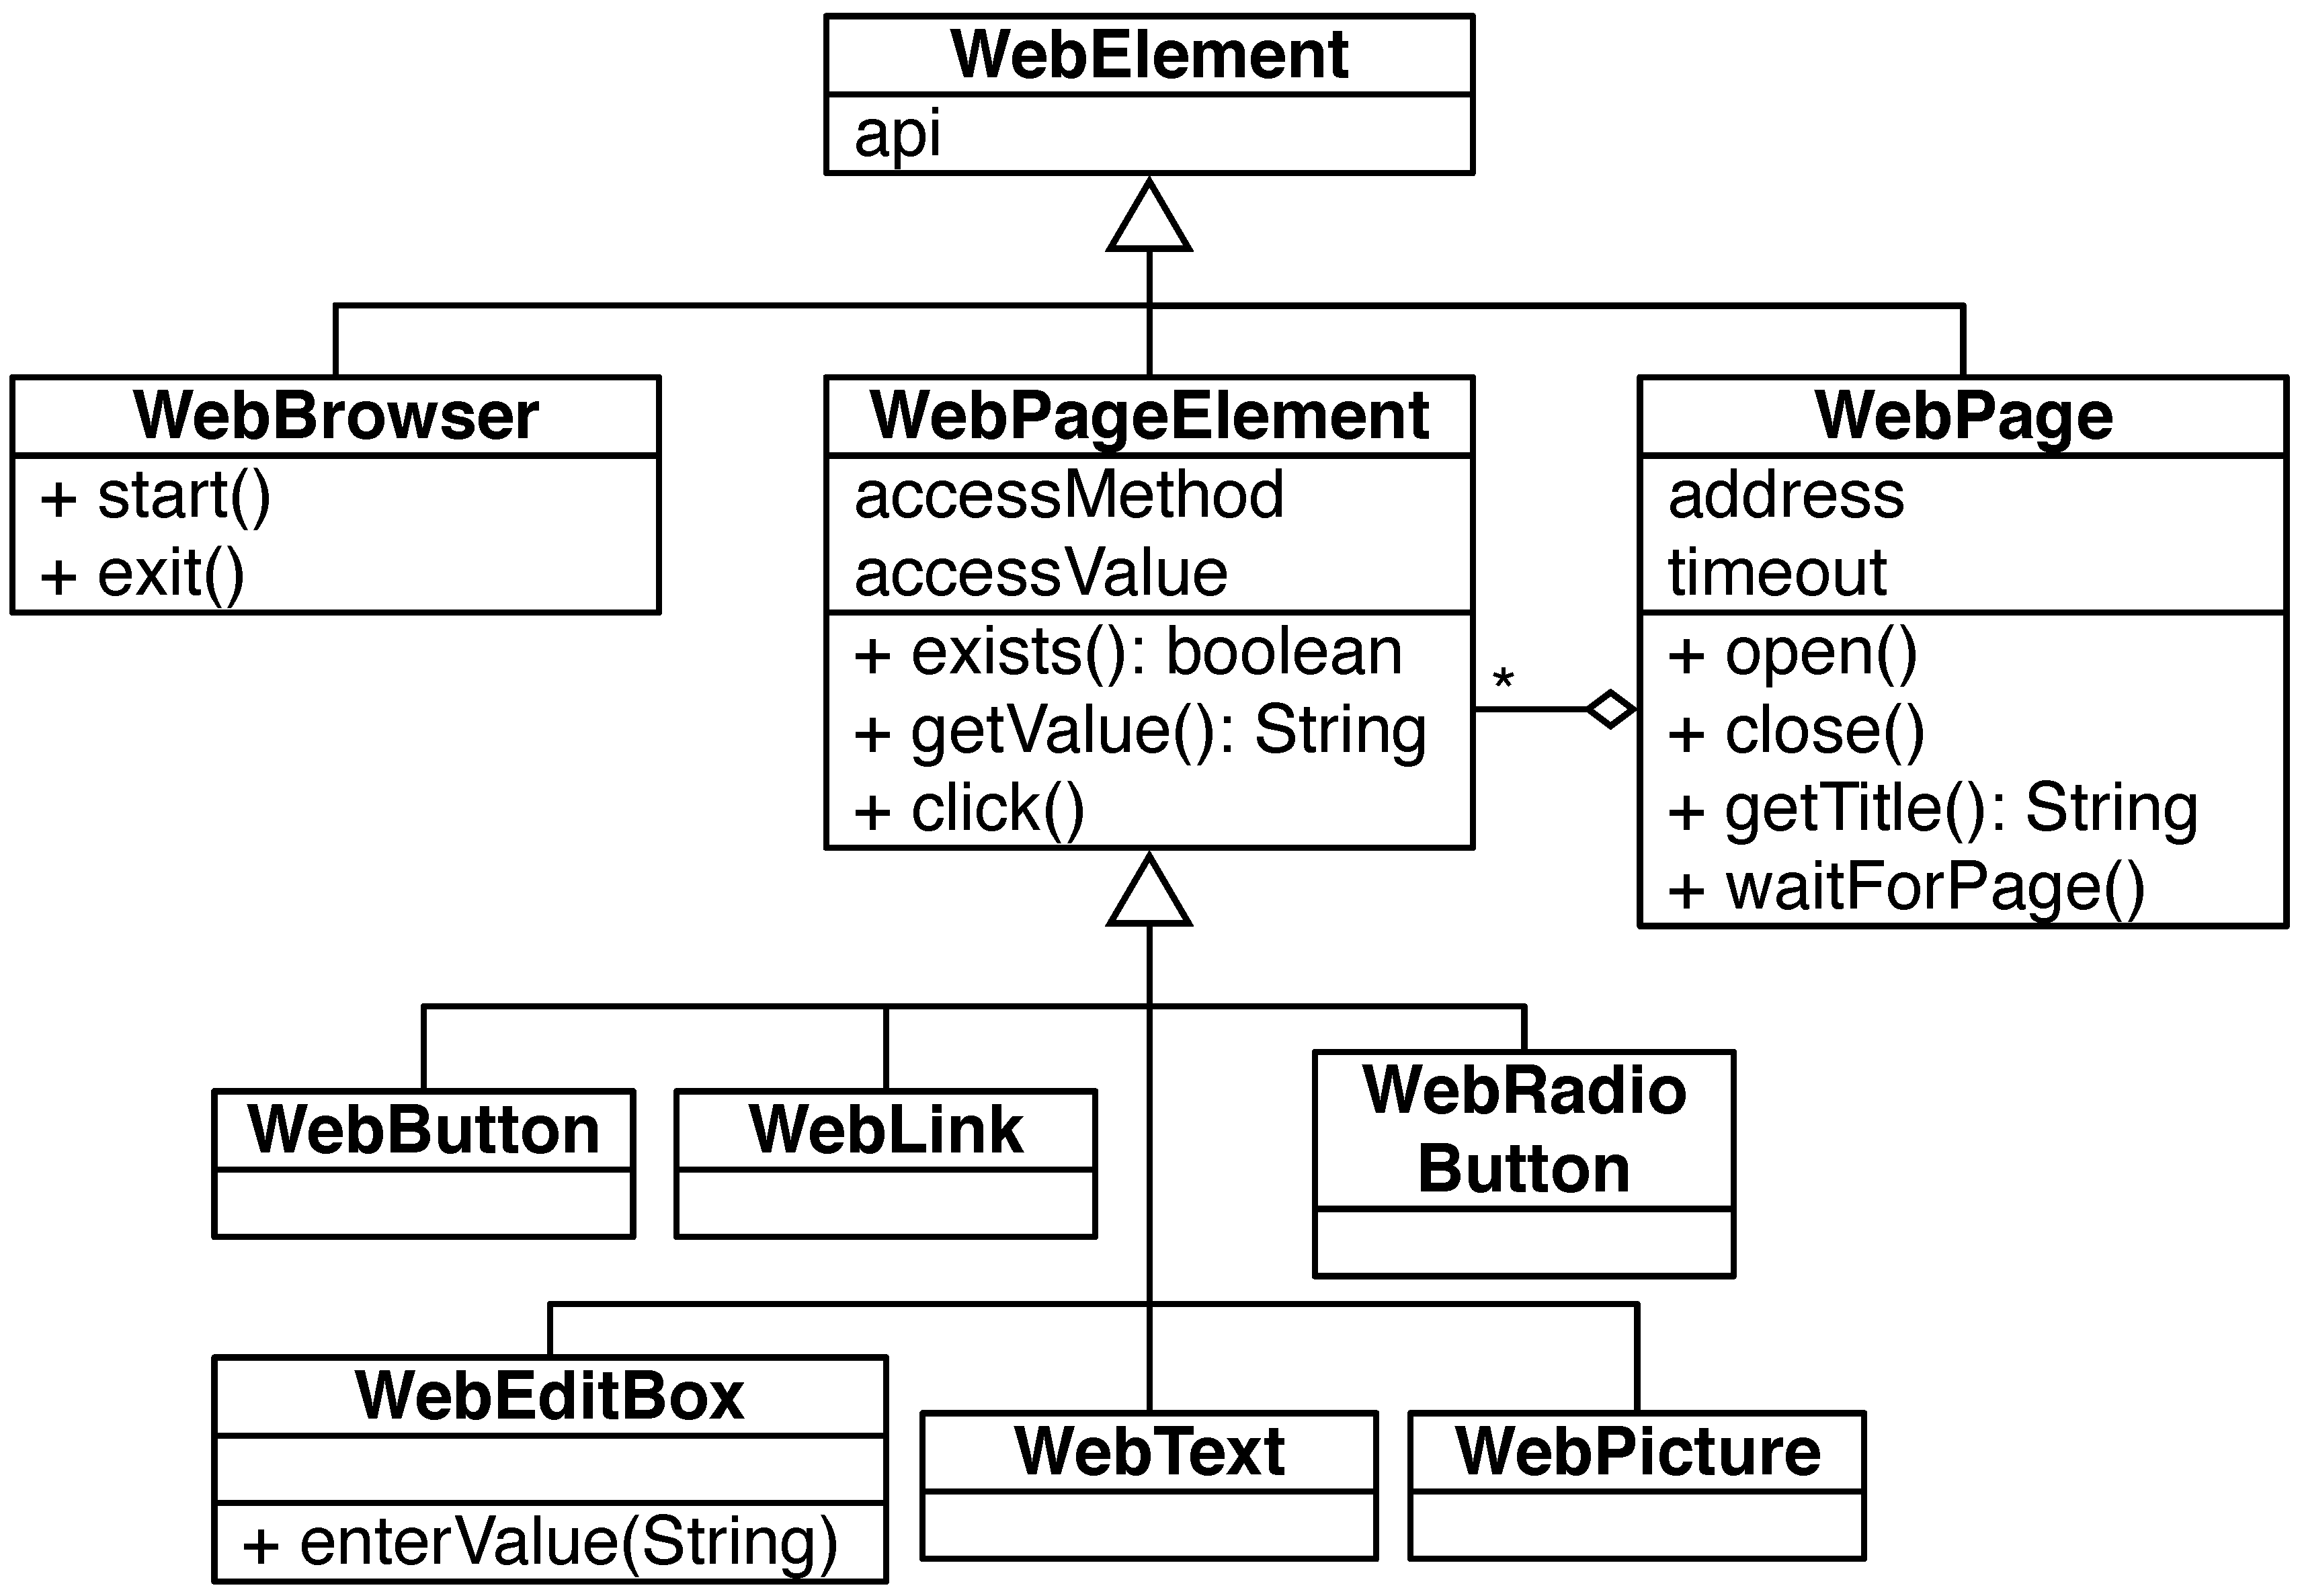
\includegraphics[width=90mm]{abscon-WebappUImodel}
	\caption{Web-applications SUT's interface class diagram (\texttt{web})}
	\label{fig:abscon:WebappUImodel}
\end{figure}

A SUT's interface model describes for a particular family of SUTs the different elements accessible when performing black-box testing. For instance, for Web-applications, the \texttt{web} model at line \ref{lst:abscon:xmltestcase:uimodel} in Listing \ref{lst:abscon:xmltestcase} is defined (here using a class diagram notation to ease the reading) in Figure \ref{fig:abscon:WebappUImodel}. It described the different elements we can found on a Web page: each class has to access the QTaste Selenium test API (using inherited attribute \texttt{api}) and will extend \texttt{WebElement};  \texttt{WebBrowser} objects will \texttt{start} and \texttt{exit} the Web browser specified for the current test case execution using the data from the external CSV file (as on line 6 in Listing \ref{lst:abscon:testcase}); a \texttt{WebPage} is available at a given URL  \texttt{address}, may be opened (and expected to load before a given \texttt{timeout}), closed, and has a title; \texttt{WebElement}s will appear on this page, each one is accessible using an \texttt{accessMethod} (\eg XPath) and an access value (\eg an XPath query to this element), may or may not exist on the page, has a value, and may be clicked;  the different elements we identified (relevant for the examples of this paper) are \texttt{WebButton}, \texttt{WebLink}, \texttt{WebRadioButton}, \texttt{WebText}, \texttt{WebPicture}, and \texttt{WebEditBox} which may be filled using textual values. 

\begin{lstlisting}[language=Python,
float,
label=lst:abscon:uimapping,
caption={Google instant search interface model instance (\texttt{UiMapping.py})}]
from uimodel_web import *

#mapping definitions
googlePage = WebPage("https://www.google.be/", 5000)
searchBar = WebEditBox("id", "lst-ib") (*@\label{lst:abscon:uimapping:searchbar}@*)
searchButton = WebButton("name", "btnK")
disableInstSearch = WebRadioButton("xpath", "//div[@id='instant-radio']/div[3]/span") (*@\label{lst:abscon:uimapping:disable}@*)
enableInstSearch = WebRadioButton("xpath", "//div[@id='instant-radio']/div[2]/span") (*@\label{lst:abscon:uimapping:enable}@*)
...
\end{lstlisting}

In AbsCon, each interface model is defined in Python. For one particular SUT's interface, this model is instantiated to represent the elements accessible to the test cases. For instance, for Google instant search, the \texttt{web} model instance is defined in \texttt{UiMapping.py} (Listing \ref{lst:abscon:uimapping}), as specified at line \ref{lst:abscon:xmltestcase:uimapping} in Listing \ref{lst:abscon:xmltestcase}. Each object is built using the dedicated constructor, which will require in most cases an access method and an access value: \eg search bar is accessed using its \texttt{id} in the page, which is \texttt{lst-ib} (line \ref{lst:abscon:uimapping:searchbar}), or using an XPath expression (lines \ref{lst:abscon:uimapping:disable} and \ref{lst:abscon:uimapping:enable}).
%
As for test APIs, interface models may be reused across different SUTs, as long as they share the same kind of interface (Web pages in this case).

%--------------------------------------------
\subsection{Assertions and actions mapping}
%--------------------------------------------

AbsCon extracts assertions and actions from the abstract test cases (Listing \ref{lst:abscon:xmltestcase}). Each assertion is mapped to a verification (\ie a function returning true or false) over the SUT's interface; and each action is mapped to a sequence of operations over elements of the SUT's interface (\ie again, a function). 

Verifications as well as operations are defined using the interface model instance defined in \texttt{UiMapping.py} (and will manipulate the different elements using the methods defined for those elements) and the QTaste data mapping mechanism in order to retrieve data from the external \texttt{TestData.csv} file. The mapping between the assertions and actions from the abstract test case is done by using the same name for the verifications and operations functions.

\begin{lstlisting}[language=Python,
float,
label=lst:abscon:operations,
caption={Verifications and operations mapping (\texttt{Operations.py})}]
from qtaste import *
from UiMappings import *

#Actions definition
def goHomePage():
	googlePage.open() 

def inputSearchString(): (*@\label{lst:abscon:uimapping:inputSearchString}@*)
	searchBar.enterValue(testData.getValue("SEARCHVALUE"))
...
#Asserts definition
def searchResultsPrinted(): (*@\label{lst:abscon:uimapping:searchResultsPrinted}@*)
	googlePage.waitForPage()
	if (not(navPicture.exists())):
		time.sleep(3) # wait for loading and retry
	return navPicture.exists()
...
\end{lstlisting}

For instance, Listing \ref{lst:abscon:operations} presents the verifications and operations mapping (\texttt{Operations.py}) for the Google instant search test cases from Listing \ref{lst:abscon:xmltestcase}. Function \texttt{inputSearchString} (line \ref{lst:abscon:uimapping:inputSearchString}) corresponds to the action with the same name in the test cases and inputs a search string, coming from the \texttt{SEARCHVALUE} column of the external CSV file, in the Google search bar defined in \texttt{UiMappings}. Function \texttt{searchResultsPrinted} (line \ref{lst:abscon:uimapping:searchResultsPrinted}) corresponds to the assertion with the same name in the test case, and returns true if the navigation picture from the result page is loaded.

%------------------------------------------------
\subsection{Test cases generation and execution}
%------------------------------------------------

Once the mappings are defined, AbsCon generates concrete (\ie executable) test cases for QTaste: for each test case, it  creates a Python script which imports the mappings and executes a sequence of \texttt{doStep} and \texttt{doAssert} calls using the verifications and operations functions. Those Python files, with the \texttt{TestData.csv} file, are used as input for QTaste to execute the test cases on the SUT and generate a summary test report.

Listing \ref{lst:abscon:testcasedef} presents the result of the generation for test case \ref{testcase1}: each \texttt{doStep} call (part of the standard QTaste API) corresponds to one action in the test case and will execute the given function. The \texttt{doAssert} function, defined by AbsCon, calls the given function (corresponding to an assertion in the test case) and prints the given error message if the call returns false. 
 
\begin{lstlisting}[language=Python,
float,
label=lst:abscon:testcasedef,
caption={Generation result for test case \ref{testcase1}}]
from qtaste import *
from Operations import *

#Assert
def doAssert(method, message):
	res = method()
	if res == 0:
		raise QTasteTestFailException(message)

#Steps
doStep(start)
doStep(goHomePage)
doAssert(onHomePage, "assertion onHomePage has failed")
doStep(inputSearchString)
doAssert(searchResultsPrinted, "assertion searchResultsPrinted has failed")
...
\end{lstlisting}


%%%%%%%%%%%%%%%%%%%%%%%%%%%%%%
\section{Implementation}
%%%%%%%%%%%%%%%%%%%%%%%%%%%%%%

\label{sec:abscon:architecture}

QTaste's plugin development functionality has been developed for specific requests made to QSpin. To the best of our knowledge, there is no plugin developer documentation available, but thanks to a QSpin developer guidance in the GitHub repository (where some examples of basic QTaste plugins are available), the development of AbsCon plugin was made possible. Basically, the plugin mechanism allows one to build his own user interface in a specific area inside the QTaste's user interface. Plugins have to be developed in Java (like QTaste) and must use the standard QTaste libraries. 

%-------------------------------------
\subsection{Graphical user interface}
%-------------------------------------

\begin{figure*}[t]
	\centering
	\subbottom[Main tab]{\label{fig:printscreen:main}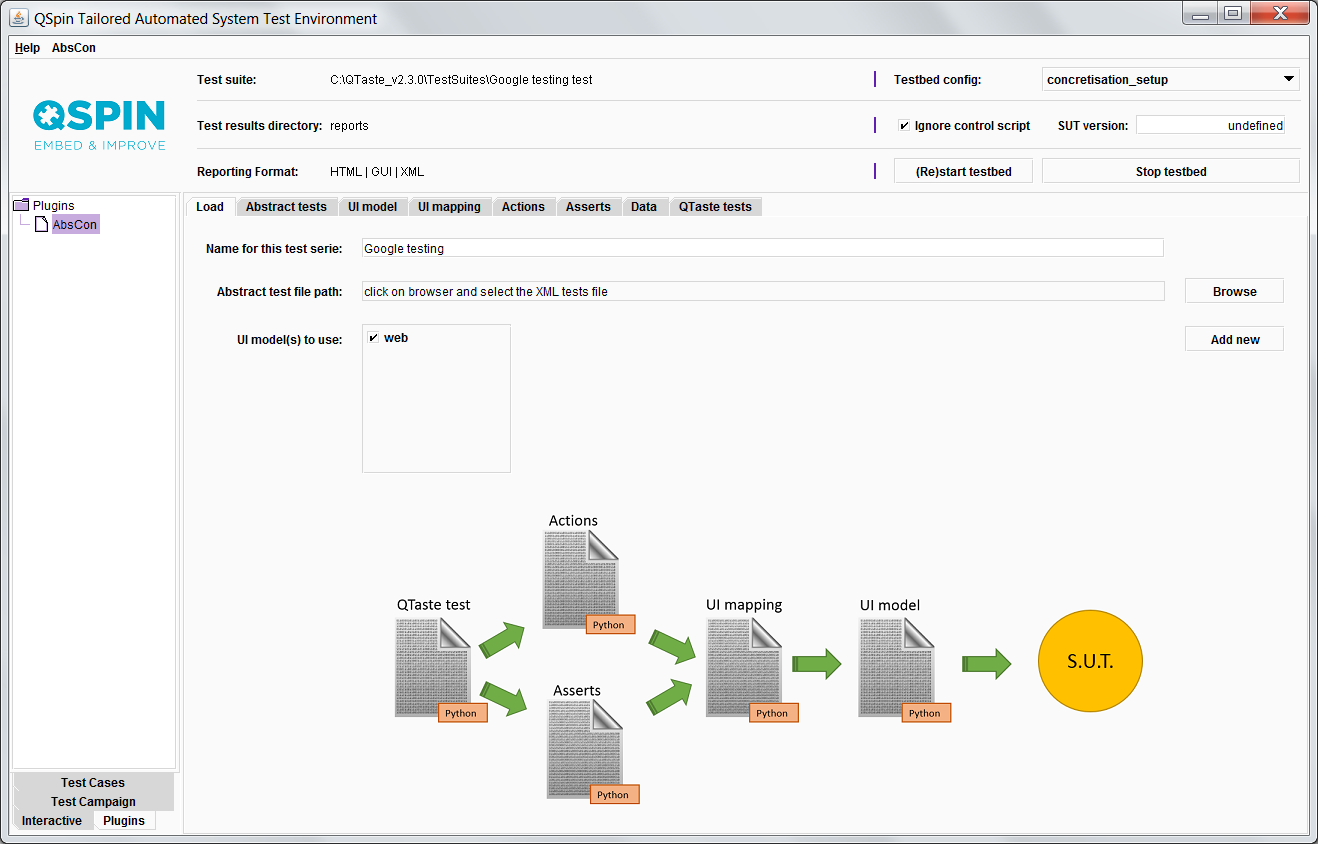
\includegraphics[width=0.99\textwidth]{abscon-main}}\\
	\subbottom[SUT interface mapping tab]{\label{fig:printscreen:uimapping}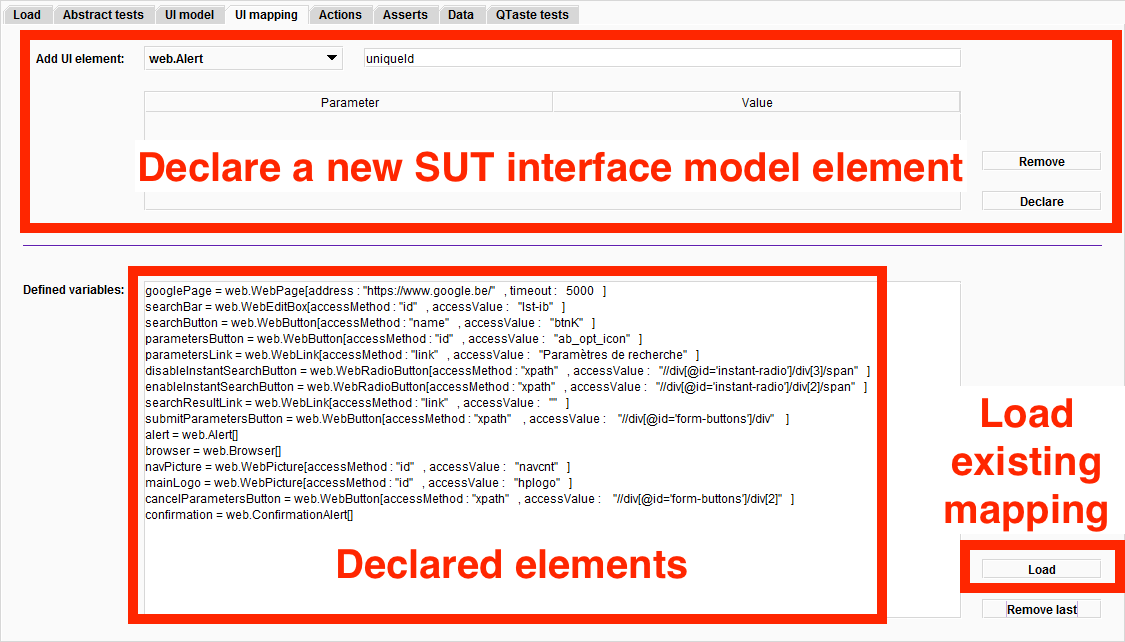
\includegraphics[width=0.44\textwidth]{abscon-uimapping}}
	\hspace{5pt}
	\subbottom[Assertions mapping tab]{\label{fig:printscreen:verifmapping}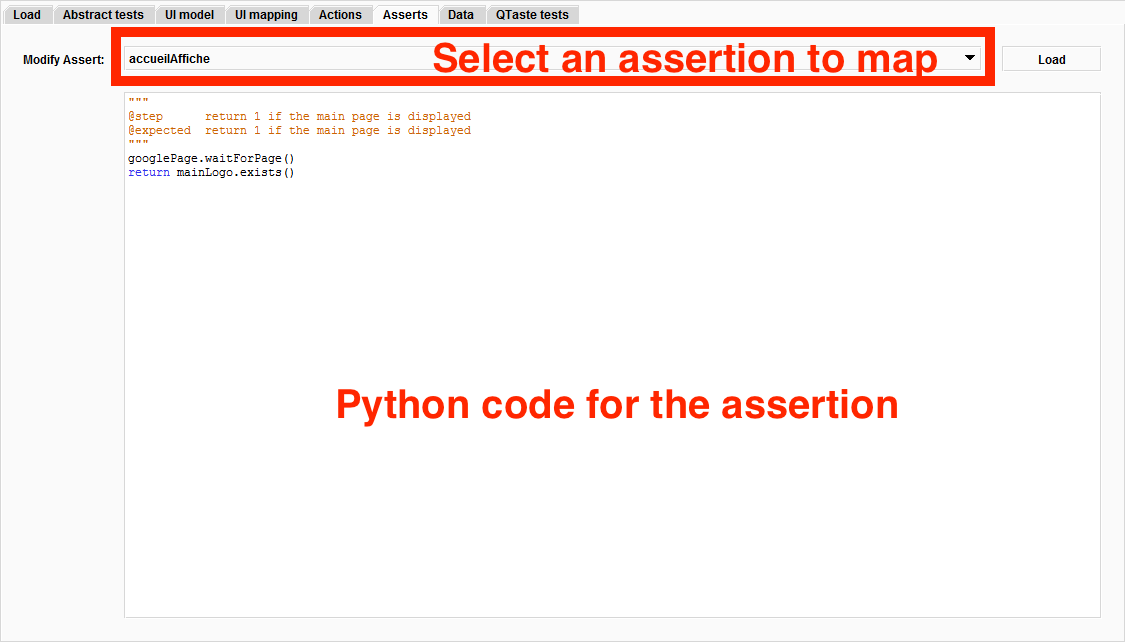
\includegraphics[width=0.44\textwidth]{abscon-asserts}}
	\caption{AbsCon plugin printscreens}
	\label{fig:printscreen}
\end{figure*}

AbsCon provides a graphical user interface integrated into QTaste (as shown in Figure \ref{fig:printscreen:main}) with different tabs, one for each mapping phase. When executing the plugin, the first step is to load the abstract test cases from an external XML file, AbsCon extracts the different actions and assertions for which a mapping has to be provided and presents them under the \texttt{Abstract tests} tab. 
The second step is to define or load a SUT's interface model (under tab \texttt{UI model}) and to instantiate this model under the \texttt{UI mapping} tab presented in Figure \ref{fig:printscreen:uimapping}: for each element of the interface, one has to instantiate a class of the interface model (selected using a drop-down list) by providing the required parameters for the constructor, and add it to the mapping using the \texttt{Declare} button (or load an existing mapping using the \texttt{Load} button). Actions and assertions mappings are given using the two next tabs: the user select the action/assertion using a drop-down list and provides the Python code for this action/assertion as shown in Figure \ref{fig:printscreen:verifmapping} (the assertion mapping tab in this case). In the \texttt{Data} tab, the user provides the data in an editable table, and finally generates the QTaste executable test cases in the \texttt{QTaste tests} tab.

%---------------------------------------
\subsection{AbsCon plugin architecture}
%---------------------------------------

\begin{figure}[t]
	\centering
	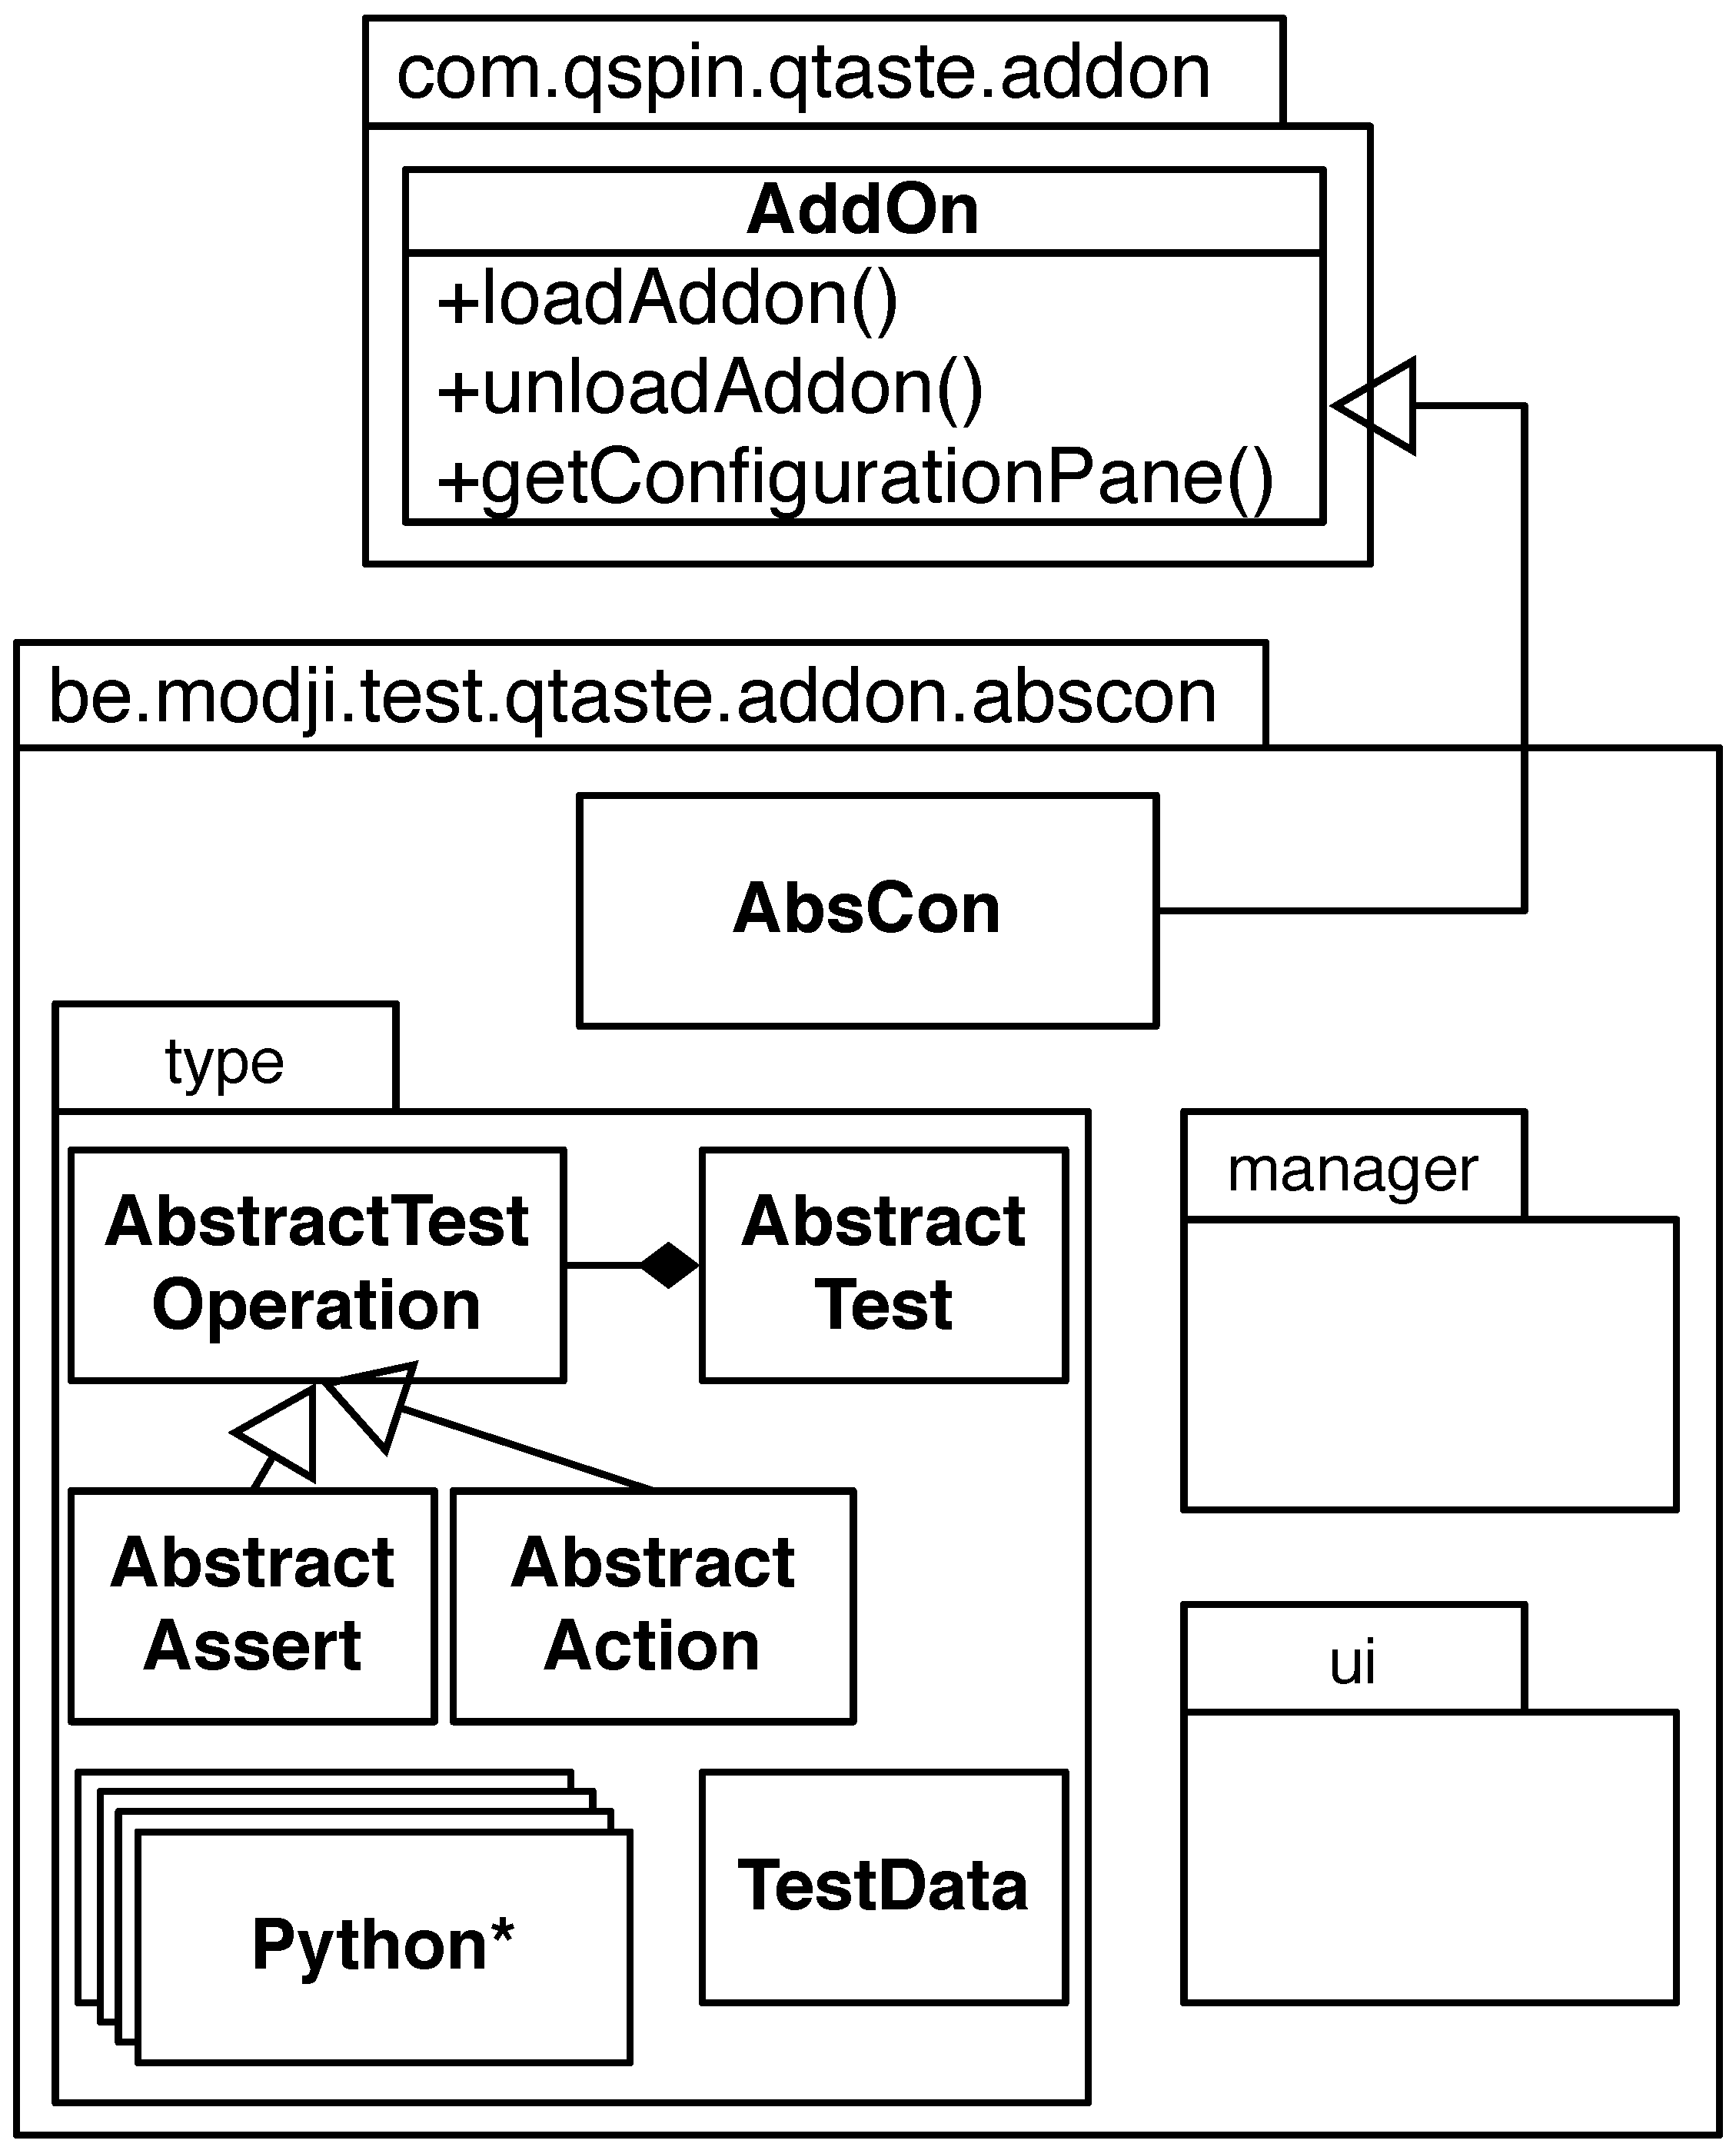
\includegraphics[width=60mm]{archi-packages}
	\caption{AbsCon packages diagram}
	\label{fig:abscon:archi-packages}
\end{figure}

Figure \ref{fig:abscon:archi-packages} gives an overview of the AbsCon packages diagram. The plugin architecture follows a classic model-view-controller pattern, divided in three Java packages: \texttt{type} one in charge of the model, \texttt{ui} package with all the classes in charge of the view, and \texttt{manager} one which contains the controller classes. 

The plugin execution is orchestrated by the \texttt{AbsCon} class, which extends the \texttt{AddOn} QTaste class: it overrides the \texttt{loadAddon}, \texttt{unloadAddon} and \texttt{get\-Confi\-gu\-ra\-tion\-Pane} methods. The two first contain all the operations to perform when QTaste loads or unload the plugin and its functionalities. The third one is the method that gives to QTaste environment the user interface of the AddOn (\ie it returns a \texttt{JPanel} that contains the plugin graphical user interface).

Model classes (package \texttt{type}) implement the different concepts presented in section \ref{sec:abscon:abscon}: abstract test cases (\texttt{AbsractTest}) are represented as a sequence of assertions (\texttt{AbstractAssert}) and actions (\texttt{AbstractAction}). The SUT's interface model and the assertions and actions mapping are encoded using Python (classes \texttt{PythonClass}, \texttt{PythonConstructor}, \texttt{PythonMethod}, and \texttt{PythonParameter}, abbreviated \texttt{Python*} in Figure \ref{fig:abscon:archi-packages}). 

Finally, the data feeding the CSV file used by QTaste during test cases execution is represented by the  \texttt{TestData} class. Manager classes (from the \texttt{manager} package) play a role of controller during the plugin execution and dialogue with the classes from the \texttt{ui} package, in charge of the AbsCon plugin graphical user interface.


%---------------------------------------
\subsection{Source code}
%---------------------------------------

AbsCon is released as an open source project on GitHub, under the GNU public license. It can be downloaded at the following address: \url{https://github.com/modji-be/AbsCon}. The project is written in Java and has 34 classes, 248 methods, and 4864 lines of code.

%%%%%%%%%%%%%%%%%%%%%%%%%%%%%
\section{Discussion}
%%%%%%%%%%%%%%%%%%%%%%%%%%%%%

\label{sec:abscon:discussion}

In this section, we discuss AbsCon's abstraction and user interface modelling mechanisms, maintenance costs, and mappings, based on our experience with the tool. A complete and rigorous evaluation of the tool, using a controlled experiment \cite{Wohlin2000} with test engineers, is left for future work.

\paragraph{Abstraction:}
%-------------------------

AbsCon heavily relies on \emph{abstraction}, of the SUT's interface on the one hand, and on the assertion and actions on the other hand. This abstraction layer allows to define each mapping independently from the higher or lower levels: abstract test cases are defined using assertions and actions with meaningful names for the user/test engineer; each assertion and each action is mapped to a Python function representing a verification or an operation, and is defined as a manipulation of the SUT's interface meaningful from a user point of view (depending on the nature of the SUT, the user may be a human or another system), thanks to the SUT's interface model; finally, the SUT's interface model encapsulates the test API calls in charge of the effective communication with the SUT. 

\paragraph{User interface modelling:}
%-------------------------------------

Another option to the modelling of the SUT's interface described in this chapter would be to use \glspl{UIDL} \cite{Guerrero-Garcia2009} such as USIXML \cite{Limbourg2005}. These languages provide generic constructs (organized in one or more metamodels that represent both platform independent and platform specific views, according to Model-Driven Architecture principles \cite{Kleppe2003})  allowing to model any kind of user-interface (including non-conventional interfaces such as voice-enabled ones). 

However, the use of such proposals in ours raises the following problem: the number of concepts they are offering being quite large, modelling a simple user interface can be cumbersome and complex, unless we tailor the language to specific needs. In our context, we do not to try to model the whole user interface but the subset concerned by the tests. We therefore adopted a lightweight approach that has the complementary advantage of not requiring any new modelling language to learn, by exploiting Python's object-orientation facilities.  Furthermore, as initially mentioned, QTaste's spectrum is larger than testing graphical user interfaces.


\paragraph{Maintenance costs:}
%-----------------------------

The goal of our abstraction layer is to reduce the overall complexity of the test cases and to decrease the \emph{maintenance costs}. Indeed, when the SUT's interface evolves, only the mapping to this interface has to be (potentially) changed, AbsCon can then re-generate concrete test cases for QTaste that will serve for non-regression. This process is much lighter than the update of QTaste test cases as it will (potentially) require to update all the test cases containing code that manipulate the SUT's interface (using directly the test API in this case). In the same way, when functionalities are added to the SUT, only the new interface elements, and verifications and operations mappings have to be added. New abstract test cases may then be written for those elements and AbsCon can re-generate a complete set of test cases for the whole SUT.

\paragraph{Mappings:}
%-------------------

The definition of the different mappings may represent an additional effort during test activities. However, different aspects have to be taken into account. First, the SUT's interface model depends solely on the nature of the SUT, \eg Web-application for the \texttt{web} model from Figure \ref{fig:abscon:WebappUImodel}. Once defined, this model may be reused across different projects. As this model abstracts the test API by defining methods from the interface point of view (\eg \texttt{click}, \texttt{open}, \texttt{getTitle}, \etc in Figure \ref{fig:abscon:WebappUImodel}), we believe that it will also soften QTaste's learning curve. Second, the definition of the mappings enables integrating existing model-based testing techniques (\eg \cite{Utting2007,vibes}) rather than defining a new complete test development process.   

In our opinion, the most time consuming task will be to \emph{identify} and \emph{map} the different SUT's \emph{interface elements}. This cost may be reduced in some cases using existing tools: for instance, \textit{Inspect} \cite{inspect}  or \textit{SwingInspector} \cite{swinginspector} are tools used to identify and access graphical user interface elements in classical desktop applications. In our \texttt{UiMapping.py} example in Listing \ref{lst:abscon:uimapping}, we used Firefox's inspection tool to identify the different elements on a Web page. Depending on the nature of the SUT, this mapping may also be partially or totally automated (this will be part of our future works), like for Web-applications for which each element on a Web page describes itself using HTML tags. 


%%%%%%%%%%%%%%%%%%%%%%%%%%%%%%%%%%%%
\section{Related work}
%%%%%%%%%%%%%%%%%%%%%%%%%%%%%%%%%%%%

\label{sec:abscon:relatedwork}

Test case \gls{concretization} techniques are classified by Utting \textit{et al.} \cite{Utting2007} in 3 categories: \emph{adaptation} approaches abstracts the SUT by using a wrapper (also called an adapter), test cases call this wrapper in order to execute operations on the SUT; \emph{transformation} approaches transform abstract test cases into test cases directly executable by the SUT, possibly using  additional information; and \emph{mixed} approaches also transform abstract test cases in executable test cases, but using an adaptation layer in order to abstract the SUT. Using this classification, QTaste uses adaptation to abstract the SUT using its test APIs and requires to write test cases which will use those test APIs. 

There exists other adapters, like \emph{Selenium} and \emph{Sahi} \cite{sahi} to test Web-applications, or \emph{AutoHotKey} \cite{ahk} to test Windows applications. Tools like \emph{Sikuli} \cite{sikuli} and \emph{Squish} \cite{squish} provide adaptation mechanisms to perform graphical user interface testing using techniques like image recognition, or recording and playback. None of these tools natively support abstract test case \gls{concretization}.

Other transformation and mixed tools like \emph{TOTEM}~\cite{Briand2001}, \emph{SpecExplorer}~\cite{Veanes2008}, \emph{MaTeLo}~\cite{Dulz2003}, \emph{Smartesting} solutions~\cite{smartesting}, or \emph{STALE}~\cite{Li2015} implement full model-based testing approaches, including abstract test case generation and concretization from different modelling languages (\eg UML Testing Profile \cite{Williams2007}, etc). 

Rather than having a complete transformation chain (from models to executable test cases), we developed AbsCon in order to plug it on an existing approach (VIBeS in this case), concretize abstract test cases, no mater their origin as long as they are described as sequences of actions and assertions, and get executable test cases on a generic and industrial test environment like QTaste.

As for VIBeS, other model-based testing approaches produce abstract test cases that are concretized using existing tools, this is the case for \emph{Skyfire}~\cite{Li2016a} which uses a transformation approach to produce \emph{Cucumber}~\cite{cucumber} abstract test cases from UML diagrams. Cucumber is a popular behaviour-driven development tool that aims at producing typical examples of the behaviour of a system under development, described using a semi-structured language: \emph{Gherkin}. Those examples are used as acceptance tests and concretized using a Java annotations based mechanism, mapping semi-structured sentences to Java methods using a defined string pattern. The executable test cases are run in standard JUnit environment. 
%
Cucumber could have been another test execution environment target, but, to the best of our knowledge, it does not provide any SUT's interface abstraction mechanism (like QTaste's test APIs) and would have required more effort to define a programmer friendly abstraction mechanism of this interface.


%%%%%%%%%%%%%%%%%%%%%%%%%%%%%%%%%%%%
\section{Wrap up and perspectives}
%%%%%%%%%%%%%%%%%%%%%%%%%%%%%%%%%%%%

\label{sec:abscon:conclusion}

In this chapter, we presented \gls{AbsCon}, a QTaste plugin developed to concretize abstract test cases represented as sequences of actions and assertions. The adaptation mechanism provided by QTaste's test API is enhanced by a programmer friendly way to encapsulate the calls to this API using a common model specific to the kind of the SUT's interface. This model, \emph{reusable} for different SUTs as long as their interface are of the same kind, defines the possible interactions with the SUTs. An instance of this model, specific to a SUT, is used in operations and verifications corresponding to actions and assertions defined in the abstract test cases. Using the different mappings, AbsCon is able to generate test cases executable in QTaste.

Originally developed to bridge the gap between VIBeS and concrete test cases, AbsCon offers multiple advantages, even in a non model-based testing context. We chose to implement it over an existing industrial test case management and execution tool, which will, we believe, eases its broader adoption. As a standalone tool (\ie not used in an model-based testing chain), AbsCon enhances QTaste's \emph{genericity} by \emph{raising the abstraction level} of different elements: the SUT's interface and test APIs, thanks to the SUT's interface model mechanism; and the test cases themselves by allowing to provide definitions using abstract actions and assertions (which is  to the user) instead of Python scripts. 

So far, the plugin has only been used on small examples, a more complete validation is part of our future works. We will also explore automated SUT's interface mapping possibilities using existing inspection tools. Finally, another potentially interesting research direction is the definition of the test cases using a structured natural language (like Gherkin \cite{cucumber}) as an input to AbsCon instead of XML files. 
This could be used to automatically define, not only the actions and assertions, but also the data to use during the test cases execution. Ideally, the definition of the test cases in a structured language would be processed by AbsCon to populate both the list of assertions and actions to map, the elements of the SUT's interface to use (based on the text describing the test cases steps), and the CSV file used by QTaste. 

More details on \gls{AbsCon} can be found in Jeremy Vanhecke's master thesis \cite{Vanhecke2016}.

